\chapter{Qt资源系统}

Qt 资源系统是一套平台独立的机制,用于将二进制文件存储至应用程序的可执行文件中。
这在您的应用始终依赖一组特定文件(如图标、翻译文件等),并且不想承担丢失这些文件的风险时,会非常有用。

资源系统基于 qmake、rcc (Qt 的资源编译器) 和 QFile 的密切协作。

\section{资源汇总文件}

通过 \hl{.qrc} 文件来指定应用程序所关联的资源,该文件基于 XML 格式,包含了磁盘中的文件列表,并为它们标注可选的别名,以供应用程序来获取资源内容。

下文为一个 \hl{.qrc} 文件范例:

\begin{lstlisting}[language=XML]
<!DOCTYPE RCC><RCC version="1.0">
<qresource>
<file>images/copy.png</file>
<file>images/cut.png</file>
<file>images/new.png</file>
<file>images/open.png</file>
<file>images/paste.png</file>
<file>images/save.png</file>
</qresource>
</RCC>
\end{lstlisting}

.qrc 文件中列举的资源文件是应用程序资源树的一部分,其中指定的路径为 .qrc 文件所在目录的相对路径。注意,列举的资源文件必须位于 .qrc 文件所在目录或其子目录。

资源数据可以被编译进二进制程序,从而在运行时可被立即获取;也可以生成为二进制文件,随后在应用程序代码中注册至资源系统。

默认情况下,资源文件在应用程序中,可使用它们在资源树中的路径,附加上 :/ 前缀来访问,也可以通过名为 qrc 的 URL Scheme 来访问。

例如,文件路径 :/images/cut.png,或 链接地址 qrc:///images/cut.png,可以用于访问 cut.png 文件,该文件在应用程序资源树中的路径为 images/cut.png。该路径也可以通过 file 标签的 alias 属性进行修改:

\begin{lstlisting}[language=C++]
<file alias="cut-img.png">images/cut.png</file>
\end{lstlisting}

此时,该文件可通过 :/cut-img.png 路径访问。也可以通过 qresource 标签的 prefix 属性为 .qrc 文件中的所有资源文件设置路径前缀:

\begin{lstlisting}
<qresource prefix="/myresources">
    <file alias="cut-img.png">images/cut.png</file>
</qresource>
\end{lstlisting}

在此场景下,该文件可通过 :/myresources/cut-img.png 路径访问。

某些资源需要随用户的区域设置发生改变,如翻译文件或图标。这可以通过在 qresource 标签中添加 lang 属性,为其指定对应的区域名称字符串来实现,例如:

\begin{lstlisting}
<qresource>
    <file>cut.jpg</file>
</qresource>
<qresource lang="fr">
    <file alias="cut.jpg">cut_fr.jpg</file>
</qresource>
\end{lstlisting}

若用户区域为法国(即 QLocale::system().name() 函数返回 "fr\_FR"),则 :/cut.jpg 会引用至 cut\_fr.jpg,其它情况下使用 cut.jpg。

\begin{seeAlso}
QLocale 文档以获取区域字符串格式的说明。
\end{seeAlso}

\begin{seeAlso}
QFileSelector 文档以了解另一个基于区域选取资源的机制,该机制可基于操作系统等更多附加信息来进行选取。
\end{seeAlso}

\section{外部二进制资源}

若要生成外部二进制资源,您需要传递 -binary 选项至 rcc 来创建资源数据文件(通常使用 .rcc 扩展名)。二进制资源文件创建完毕后,可以通过 QResource 接口进行注册。

例如,.qrc 文件中指定的一组资源数据,可以通过如下方式进行编译:

\begin{lstlisting}
rcc -binary myresource.qrc -o myresource.rcc
\end{lstlisting}

在应用程序中,通过如下代码注册资源:

\begin{lstlisting}[language=C++]
QResource::registerResource("/path/to/myresource.rcc");
\end{lstlisting}

\section{内建资源}

若要将资源编译至二进制程序内,您需要在应用程序的 .pro 文件中指定 .qrc 文件,从而让 qmake 可以感知到它。例如:

\begin{lstlisting}[language=C++]
RESOURCES     = application.qrc
\end{lstlisting}

\hl{qmake} 会生成编译规则来创建名为 \hl{qrc\_application.cpp} 的源文件,并将其链接至应用程序。

该文件包含以 C++ 静态数组的形式存储的图片和其它所有资源的二进制压缩数据。

\hl{qrc\_application.cpp} 文件会在 \hl{.qrc} 文件或其引用的任意资源文件发生改变时自动重新生成。

若您不使用 \hl{.pro} 文件,则需要手动执行 \hl{rcc},或将其添加到您的构建系统中。

\begin{figure}[hbt!]  
	\centering
    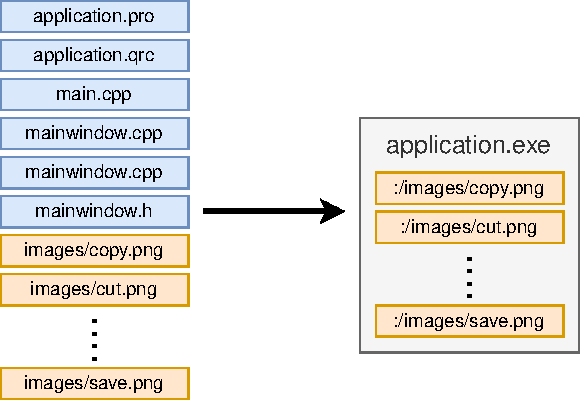
\includegraphics[width=0.5\textwidth]{The_Qt_Resource_System}
\end{figure}

目前,Qt 总是将数据直接存储至可执行程序内,无论是 Windows、macOS 还是 iOS——这些操作系统都提供了内嵌资源的原生支持。这个模式在 Qt 未来的版本中可能会有改变。

\section{压缩}

\hl{rcc} 会尝试压缩资源数据来减少最终生成的二进制文件的磁盘占用。
通常情况下,会通过启发式的检查来决定是否值得进行压缩,并且在无法有效压缩的情况下直接存储未压缩的内容。
您可以使用 \hl{-threshold} 来控制判断阈值,该选项告知 \hl{rcc} 源文件压缩后获得的体积缩减必须不小于该百分比。

\begin{lstlisting}[language=C++]   
rcc -threshold 25 myresources.qrc
\end{lstlisting}

默认值为 \hl{70},意味着压缩后的文件必须比源文件小 70\%(即不大于源文件的 30\% 大小)。

若有需要的话,也可以关闭压缩,这在资源文件中包含已经压缩过的数据时(如 \hl{.png} 文件)非常有用——否则会在编译时浪费 CPU 时间来确认它的确不能被再次压缩。
另一个原因则是无需考虑磁盘占用,并且想让资源在运行时以可直接访问的原始数据存放于内存中,而非需要解压才可使用的压缩数据。
您可以通过命令行参数 \hl{-no-compress} 来实现此目的。

\begin{lstlisting}   
rcc -no-compress myresources.qrc
\end{lstlisting}

\hl{rcc} 同样给予用户控制压缩算法和压缩等级的权限,例如:

\begin{lstlisting}[language=C++]   
rcc -compress 2 -compress-algo zlib myresources.qrc
\end{lstlisting}

另外,也可以在 \hl{.qrc} 文件中 \hl{file} 标签的 \hl{threshold}、\hl{compress} 和 \hl{compress-algo} 属性来进行设置:

\begin{lstlisting}[language=XML]  
<qresource>
    <file compress="1" compress-algo="zstd">data.txt</file>
</qresource>
\end{lstlisting}

上述代码选择 \hl{zstd} 算法,使用压缩等级 1.

\hl{rcc} 支持如下压缩算法和压缩等级:

\begin{compactitem}[\arr]
\item \hl{best}:使用下述算法中的最优者,并使用其最高压缩等级,以编译时的 CPU 时间为代价来获得最高压缩率。
    此参数在 XML 文件中可用于指明无论 \hl{rcc} 支持何种压缩算法,该文件都应被尽可能地压缩。
\item \hl{zstd}:使用 Zstandard 库进行压缩。有效压缩等级为 1 至 19,1 为最低压缩率(最短 CPU 时间),19 为最高压缩率(最长 CPU 时间)。
 默认等级为 14。特殊值 0 用于告知 \hl{zstd} 库自由选择其默认的压缩率。
\item \hl{zlib}:使用 zlib 库进行压缩。有效压缩等级为 1 至 9,1 为最低压缩率(最短 CPU 时间),9 为最高压缩率(最长 CPU 时间)。
    特殊值 0 代表“无需压缩”,并且不应被使用。默认值为实现定义,通常为 6。
\item \hl{none}:无压缩。该参数等价于 \hl{-no-compress} 选项。
\end{compactitem}

Zstandard 和 zlib 均为可选支持。若运行时未检测到对应的库,则通过 \hl{-compress-algo} 指定该库的操作会报错。
默认情况下,若 \hl{zstd} 可用则使用该算法,否则使用 \hl{zlib}。

\section{在应用程序中使用资源}

在应用程序中,资源路径可用于绝大多数常规文件系统路径的中。
例如,可以传递资源路径而非文件路径至 QIcon,QImage 或 QPixmap 的构造函数:

\begin{lstlisting}[language=C++]
cutAct = new QAction(QIcon(":/images/cut.png"), tr("Cu&t"), this);
\end{lstlisting}

\begin{notice}
Application 范例以了解实际程序中如何使用 Qt 的资源系统来存储图标。
\end{notice}

资源在内存中以资源对象树形式表达,该对象树在程序启动时构建,通过 QFile 来将其路径解析至资源数据。
可通过 \hl{":/"} 初始化 QDir 对象,来从根部遍历该对象树。

Qt 的资源系统支持搜索路径列表概念。若通过 \hl{:} 而非 \hl{:/} 前缀来指定资源,则会通过搜索路径列表来检索该资源。
搜索路径列表在程序启动时为空,可通过 QDir::addSearchPath() 来添加路径。

\section{使用库中的资源}

若在库中包含资源,则需要调用 Q\_INIT\_RESOURCE() 来强制初始化资源,调用参数为 \hl{.qrc} 文件的基本名称,例如

\begin{lstlisting}[language=C++]
MyClass::MyClass() : BaseClass()
{
    Q_INIT_RESOURCE(resources);

    QFile file(":/myfile.dat");
    ...
}
\end{lstlisting}


这确保了在静态链接时,资源数据可被链接至最终的应用程序。
该初始化代码应该紧贴在库中使用资源的位置之前,以确保仅当该库的使用者使用到依赖资源的特性时,才会将资源链接至程序。

\begin{notice}
由于 \hl{rcc} 生成的资源初始化器定义在全局命名空间,Q\_INIT\_RESOURCE() 的调用也必须位于任何命名空间之外。
\end{notice}

若该库包含的资源不在内部使用,而是暴露给库的使用者,则初始化操作需要发生在应用程序代码中,例如:

\begin{lstlisting}[language=C++]
int main(int argc, char *argv[])
{
    QApplication app(argc, argv);
    Q_INIT_RESOURCE(graphlib);
    
    QFile file(":/graph.png");
    ...
    return app.exec();
}    
\end{lstlisting}

如上文所述,此方式确保了资源数据可在静态链接时被链接至最终的应用程序,同时也会在动态链接时触发库的加载动作,如加载插件。

类似地,若想显示地卸载一组资源(因为需要卸载插件,或该资源不再被使用),则可通过调用 Q\_CLEANUP\_RESOURCE() 来强制移除资源,调用参数与上文相同。

\begin{lstlisting}
若资源文件被编译为应用程序的一部分,则不需要使用 Q\_INIT\_RESOURCE() 和 Q\_CLEANUP\_RESOURCE()。
\end{lstlisting}